\chapter{Technical Approach}\label{chapter:tech}
\section{System Overview}
Figure \ref{fig:sys_overview} provides a high-level overview of the system architecture. The system consists of several microservices, each of which perform a unique function. 

The client facing side, the ‘front-end’, of the application, displayed in yellow (see \ref{fig:sys_overview}), consists of Productizer and Grunt. The Productizer provides a graphical interface through which the user can interact with the system, providing training data from uploaded images to the back-end of the system, and adding images that require classification in batches to the Amazon Simple Queue Service (SQS) queue. The queue worker, Grunt, takes images from the SQS queue and sends them to the back-end for processing, writing their classifications to the front-end database, and publishing notifications to PubNub when a task has been processed.

The server side, or ‘back-end’ of the application, displayed in blue (see \ref{fig:sys_overview}), consists of Saturn, Olivia and the Classifier. Saturn acts as the central point of communication, forwarding requests to Grunt, Olivia and the Classifier. Olivia is responsible for downloading images and extracting a 1024-attribute vector from them. The Classifier uses these vectors to predict the class of the image.

\begin{figure}[H]
    \centering
    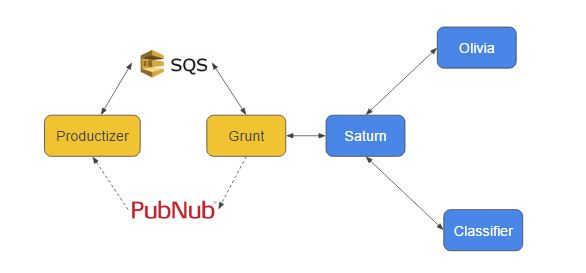
\includegraphics[width=\textwidth]{figs/4/sys_overview}
    \caption{High-level overview of the system architecture}
    \label{fig:sys_overview}
\end{figure}

\section{Requirements}
Before beginning development, requirements were gathered based on the requests of the customer and the needs of the system, details of which are outlined below.
\subsection{Functional Requirements} \label{funcreqs}
\subsubsection{Image Uploading}
The user will be able to upload any Ordnance Survey aerial image. These images could be of any size, and across a range of qualities.
\subsubsection{Feature Selection}
The user will be able to select any feature visible on the image. Despite using tiling, the user will be able to select features that sit on the borders of two tiles. 
\subsubsection{Attribute Extraction}
The system will extract information from selected features, allowing them to be identified.
\subsubsection{Feature Identification}
The system will use classification algorithms, trained with supervised training data gathered by the user, to identify features based on the extracted information.
\subsubsection{Iterative Training}
The user will be able to iteratively train the system over time by providing additional training data for existing classes and new ones. 
\subsubsection{Intuitive Interface}
The system will have an intuitive interface that will be used to train the classifier and obtain its predictions, while hiding the complexity of the program from the user, such that no knowledge or experience with classification algorithms is required.

\subsection{Non-Functional Requirements} \label{nonfuncreqs}
\subsubsection{Accuracy}
After sufficient training, the system will be capable of classifying features with an overall accuracy of 80% or more.
\subsubsection{Scalability}
The system will be capable of identifying 100 unique features without significant reduction in performance.
\subsubsection{Speed}
The system will process each 256x256 tile of an image in under 0.1s.
\subsubsection{Usability}
Using the user interface, the user will be able to provide the system with sufficient training data to identify a new class under 5 minutes.
\subsubsection{Productivity}
Over a substantial period of time, an experienced user of the system will have higher levels of productivity (i.e a faster rate of feature identification) compared to that same user identifying features manually.

\subsection{Implementation Requirements} \label{impreqs}
\subsubsection{Language}
\subsubsubsection{Front-end} \label{frontendlang}
The front-end application must allow for communication with a MySQL database, as well as provide the ability to serve a HTML/CSS based website. The application must be able to run front-end JavaScript in order to provide support for Google Maps API, allowing image manipulation. Furthermore, the application should allow the uploading and retrieval of images that can be used within the map display. 
\subsubsubsection{Back-end} 
The back-end language must allow for fast development, with access to relevant third-party module, such as classification algorithms and HTTP communication libraries. Additionally, it should be compatible with Olivia’s attribute extraction code, which was written in Python.
\subsubsection{Persistence}
\paragraph{Front-end\\}
Persistence is used in the front-end to:
\begin{itemize}
    \item Store initial uploaded image, and all tiles generated from this
    \item Store maps in database with unique ID, link to image path, and further details
    \item Store tiles in database, associated with specific map, along with their coordinates and classifications
\end{itemize}
\paragraph{Back-end\\}
Persistence is used in the back-end to:
\begin{itemize}
    \item Map image IDs to extracted attributes in the Attribute Extractor
    \item Store all training data in the classifier microservice
    \item Map Feature ID Number to Feature Name in the classifier
\end{itemize}
\subsubsection{Front-end}
The front-end of the application must be accessible by multiple users concurrently from any location. 
\subsubsection{Platform}
The back-end of application must run on a platform that makes it available to a wide audience.
\subsubsection{Framework}
The framework must be quick to learn due to the limited time available. Only basic utility is required from the framework for the purposes of this project. The two main options available in Python are Flask and Django. 
\subsection{Interface Requirements} \label{intreqs}
\subsubsection{Image Manipulation}
The interface will allow the user to upload any Ordnance Survey aerial image, pan around the image and select any visible feature on the image. It should also provide quick access to previously uploaded images. 
\subsubsection{Interaction with Classifier}
The interface will allow the user to interact with classifier, providing supervised training data for existing and new classes, and obtaining the its predictions. The interface will be simple and easy to use, hiding the complexity of the classification algorithm, such that no experience in machine learning is required.
\subsection{Use Case Analysis}
Figure \ref{fig:comic} was produced during the initial use case analysis of the project, providing a high-level overview of the functionality required by the system.
\begin{figure}[H]
    \centering
    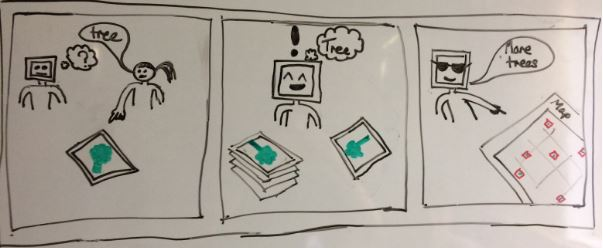
\includegraphics[width=\textwidth]{figs/4/comic}
    \caption{A comic strip produced to provide a high-level overview of system functionality}
    \label{fig:comic}
\end{figure}

Following this comic strip, a formal use case diagram was produced, as shown in figure \ref{fig:use_case_diagram}. As shown in the diagram, users will be able to upload their own map or work on previous maps. They can then select Learn Mode and train the classifier by selecting features and providing their true class, or select Discover Mode and obtain the classifier’s predictions, filtering the output to show the feature they are looking for. They can create new classes, and after providing sufficient training data, reclassify the map to find occurrences of this new feature.  
\begin{figure}[H]
    \centering
    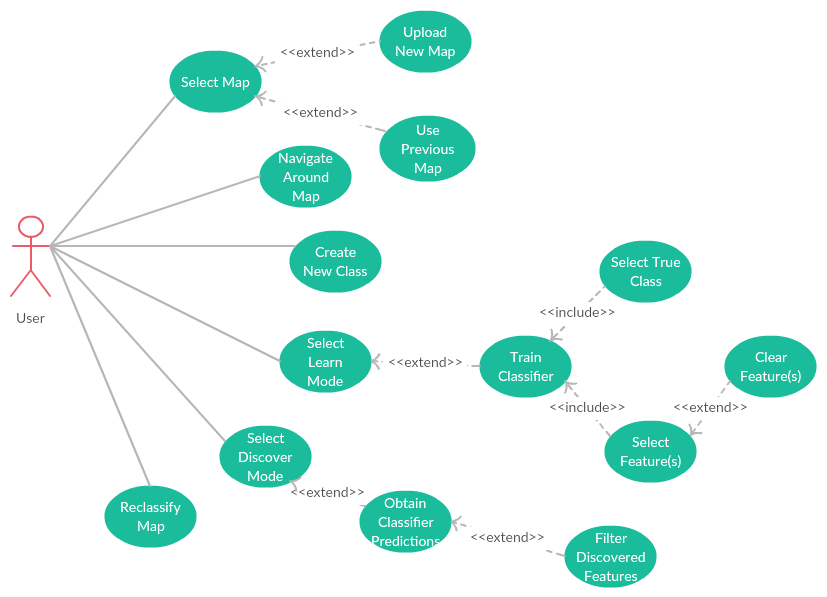
\includegraphics[width=\textwidth]{figs/4/use_case_diagram}
    \caption{The System Use Case Diagram}
    \label{fig:use_case_diagram}
\end{figure}

\section{Design}
\subsection{Overview}
Having considered the system requirements, a number of design choices were made to ensure the system met these requirements. 
\subsection{Design Choices}
\subsubsection{Language}
\paragraph{Front-end\\}
PHP was used to ensure all of these requirements outlined in \ref{frontendlang} are met. Additionally, PHP provides a vast community of developer support and a number of pre-built frameworks that can enhance speed of development.
\paragraph{Back-end\\}
Python was chosen as the back-end development language due to the fast code development and vast quantity of third-party support offered. Additionally, using Python ensures compatibility with Olivia’s attribute extraction code, allowing for flexibility in the system architecture. 
\subsubsection{Persistence}
\paragraph{Front-end\\}
All images are stored in the application file system to maintain front-end persistence. In order to store the map and tile details, a MySQL database was used in order to create a relational database that could link the tiles with their associated map. PHP provides secure functions to interact with MySQL databases to negate the risk of SQL injection, plus frameworks such as Laravel provide Object-relational mapping to allow abstraction from direct SQL queries.
\paragraph{Back-end\\}
CSV files were used for the back-end persistence, since a simple storage system with read-all and write-all functions is all that was required. Python supports this method of storage with a CSV module, providing all required functions. Additionally, this approach is lightweight and easily implemented. 
\subsubsection{Front-end}
A cloud-hosted web application was used for the user interface of the application, allowing it to be accessed by multiple users concurrently.
\subsubsection{Platform}
The back-end of the application was designed to ensure it could be run on Linux. 
\subsubsection{Framework}
Flask was selected over Django as the framework for the project. While Django is more powerful, this comes at the price of a steeper learning curve, whereas Flask supports all of this project’s requirements and also can be learnt relatively quickly.
\subsection{Iterations}
\subsubsection{Iteration 1}
\paragraph{Overview\\}
While using an agile methodology, it is important to ensure that a minimum viable product is developed by the end of each iteration. Based on this concept, the following simple client-server architecture was implemented during the first iteration (Figure \ref{fig:iteration1_overview}). 
\begin{figure}[H]
    \centering
    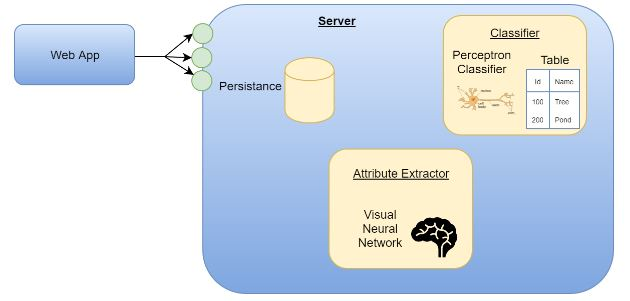
\includegraphics[width=\textwidth]{figs/4/iteration1_overview}
    \caption{An overview of the client-server architecture implemented in Iteration 1}
    \label{fig:iteration1_overview}
\end{figure}
\paragraph{Client Side\\}
On the client side, a fully-functional GUI was developed, allowing the user to upload any map, access previously uploaded maps, and zoom and pan around the map. Tiling was used, splitting the map into 256x256 pixel tiles, allowing the user to select features by clicking its nearest tile.
\paragraph{Server Side\\}
On the server side, image attribute extraction was performed using code from previous student Olivia Wilson’s Masters project. This code was run on the CPU, providing a slow but functional extraction of 1024 attributes from each 256x256 tile.

To perform this extraction, the image must first be downloaded onto the server. Therefore, memory persistence was used to store images until they have been processed.

Additionally, a Perceptron was implemented as a proof-of-concept classifier. This used the extracted attributes either for supervised training or to provide basic predictions. It made use of a table to convert human-readable feature names to perceptron-useable ID numbers. 
\paragraph{Functionality\\}
These components were used to develop a product capable of two modes: Learn Mode and Guess Mode.

In Learn Mode, the user would upload an image, select a number of tiles containing features, provide the name of the feature, and click ``learn”. A HTTP POST request containing the URLs of the selected tiles was sent to the server. The server downloaded the images from the given URLs and extract their attributes into a vector. Additionally, the feature name was converted to an ID number using the lookup table. Finally, the perceptron was trained using the vectors and class ID number via supervised learning.

In Guess Mode, the user would upload an image, select a single tile, and click ``guess”. Again, on the server side the image was downloaded and its attributes extracted. The perceptron then guessed the class ID of the tile based on its attribute vector, converted this ID to a string using the lookup table, and returned the guess. The web application then displayed the predicted class to the user.

\subsubsection{Iteration 2}
\paragraph{Overview\\}
After developing a broad yet shallow product in iteration 1, the focus of iteration 2 was to add depth to the system. The client-server architecture was improved through the addition of microservices, as shown below (Figure \ref{fig:iteration2_overview}).
\begin{figure}[H]
    \centering
    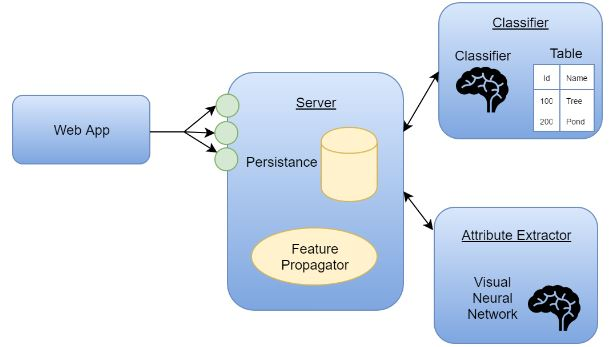
\includegraphics[width=\textwidth]{figs/4/iteration2_overview}
    \caption{An overview of the microservices architecture implemented in iteration 2}
    \label{fig:iteration2_overview}
\end{figure}
\paragraph{Web Application\\}
The web application was improved through the inclusion of Amazon SQS and PubNub. The web app now adds each image-to-be-processed to the SQS queue. The queue worker, Grunt, retrieves images from this queue and forwards them to the back-end. After an image has been processed and classified, Grunt publishes the image along with its classification results to PubNub. The web app displays PubNub classifications on the map, allowing the user to identify features of a selected class. Additionally a completion bar was displayed, showing the progress of image processing based on entries remaining in the SQS queue.
\paragraph{Server\\}
The functionality of the server was moved into separate microservices, and its responsibility was now to act as the central point of communication between microservices. Additionally, it contained global data persistence for the classifier and attribute extractor, as well performing the logic used for feature finder (discussed in \ref{ittwo-classifier}) by filtering out irrelevant classes. 
\paragraph{Attribute Extractor\\}
The attribute extractor was now running as an independent microservice, hosted on a powerful machine with a GTX Titan X GPU, containing 3072 cuda cores and 12GB ram. To take advantage of this, the code was modified to run on the GPU rather than CPU. Running on the CPU, the code would take approximately 30 seconds to process a single 256x256 image, whereas on the GPU it could process a batch of 128 images concurrently in 0.1 seconds, reducing processing time by a scale of 38,400. 
\paragraph{Classifier\\} \label{ittwo-classifier}
Also now running as an independent microservice, the classifier saw a number of improvements. The perceptron algorithm used was replaced with a Support Vector Machine. This algorithm provides significantly more accurate predictions with much less training data required (see section 8 for a full list of advantages and limitations). Additionally, knowledge persistence was implemented in the classifier, storing all supervised training data it uses. This allows the classifier to learn iteratively by incrementally adding data to the storage, as well as enabling its knowledge to be easily controlled, since sub-optimal training data can be deleted and forgotten.
\paragraph{Functionality\\}
The changes listed above resulted in a number of non-functional improvements to the system: greater concurrency reducing overall processing time, faster image processing, greater prediction accuracy. Additionally, the functionality of the system was improved. 

The proof-of-concept Guess Mode implemented in iteration 1 was extended into Discover Mode in iteration 2. Rather than guessing the class of a single tile selected by the user, Discover Mode gathers the predicted class of all tiles in an image. The user can then select the feature they wish to discover, and all identified occurrences of that feature are highlighted on the map. 

\subsubsection{Final Iteration}
\paragraph{Overview\\}
By the end of iteration 2, the developed system met the specification outlined at the start of the project. The final iteration was used predominantly for bug fixes, usability testing, improvements and extensions. 
An overview of the final architecture of the system can be seen below (figure \ref{fig:iteration3_overview}).
\begin{figure}[H]
    \centering
    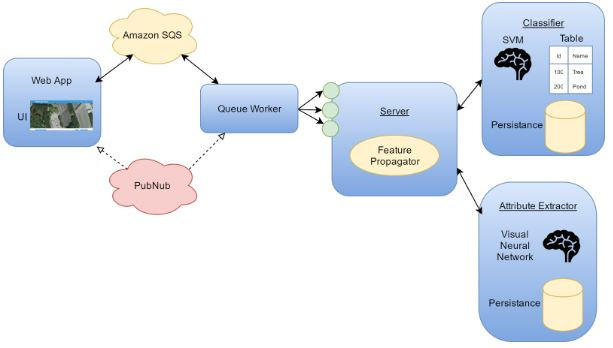
\includegraphics[width=\textwidth]{figs/4/iteration3_overview}
    \caption{An overview of the finalised architecture of the system}
    \label{fig:iteration3_overview}
\end{figure}

\paragraph{Web Application\\}
Following the feedback from usability testing, a number of improvements were made to the web application.

A highlighting square was added to the map display, outlining the boundary of the selected tile. This was used in Learn Mode to help the user to select the correct tile, and Discover mode to provide context to feature markers by showing the tile they correspond to. 

Additionally, by using 256x256 tiles, occasionally a feature would sit on the boundary between two tiles, making it unselectable. Therefore, the tiling system was revised to instead combine four adjacent 128x128 tiles to generate the 256x256 tile. This resulted in overlapping 256x256 tiles, allowing previously unselectable features to be selected. 

Finally, discover mode was improved by using a checkbox for the classes to be discovered, allowing multiple classes to be selected and discovered at once. To visualise this clearly, a different coloured marker was used for each class.  

\paragraph{Attribute Extractor\\}
Previously, the attribute extractor would download every tile image before extracting its attributes, and would often need to process the same tile multiple times. However, downloading images is the most significant bottleneck in system performance, and the extracted attributes never change for the same image.

Therefore, each tile was assigned an ID number based on its map ID, X coordinate and Y coordinate. After downloading a tile image and extracting its attributes, this vector is stored in a table, with the ID number as the key. Whenever a tile requires processing, the attribute extractor first checks for its ID number in the table, returning the corresponding attribute vector if it exists. This ensures each tile is only downloaded and extracted at most once. 

Additionally, a problem with Olivia’s attribute extraction code is that, given a 256x256 image, it only classifies the central pixel, using the surrounding 192x192 pixels as context, and ignoring the outer 32 pixel border. To solve this, the focus of the classification was shifted to 9 positions around the centre of the image, allowing for full coverage. Classification was obtained at each position, allowing probabilities to be calculated based on the distribution of predictions. 
\paragraph{Functionality\\}
As all the functional requirements system were achieved by the end of iteration 2, this final iteration was focused on achieving the non-functional requirements of the system, hence no additional functionality was added.

\subsubsection{Interaction Diagram}
The Interaction Diagram below (figure \ref{fig:interaction_diagram}) shows the interactions between microservices when the user uploads a new map.

The web application splits the image into a number of 256x256 tiles. The URLs of these tiles are sent to Saturn, which forwards them to Olivia to obtain the vector of 1024 attributes. Saturn then forwards the attributes to the Classifier, which returns a predicted class for each tile. These predictions are returned to the web application, where they are displayed on the map to the user. 
\begin{figure}[H]
    \centering
    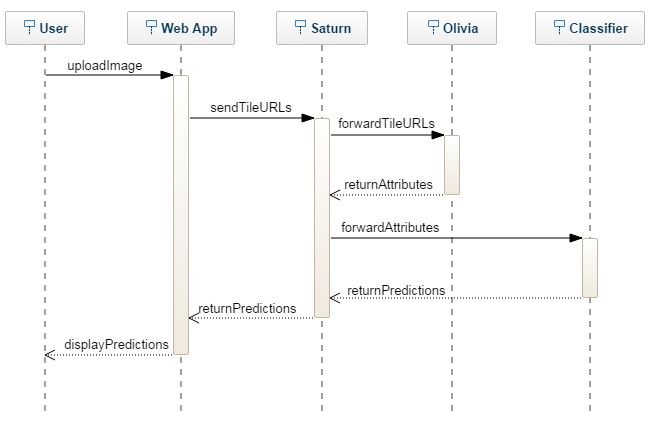
\includegraphics[width=\textwidth]{figs/4/interaction_diagram}
    \caption{An Interaction Diagram showing the process that occurs when the user uploads a map image}
    \label{fig:interaction_diagram}
\end{figure}

\subsubsection{Entity Relationship Diagram}
The following entity relationship (ER) diagrams show the entities that exist within each microservices of the system, the attributes of these entities, and the relationships between them.
\paragraph{Web Application\\}
Figure \ref{fig:webapp_er} shows the entities present in the web application. Starting with a map, a number of tiles are generated, and identified from the map ID, and the X and Y coordinates of the tile on the map. 
\begin{figure}[H]
    \centering
    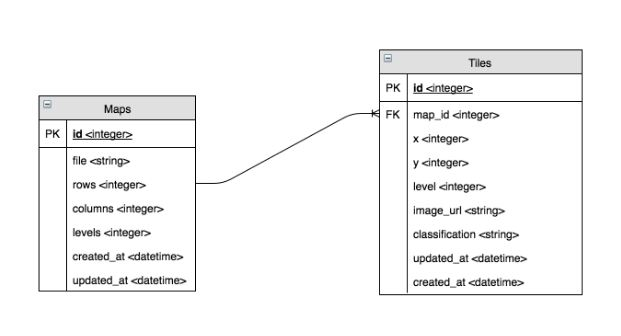
\includegraphics[width=\textwidth]{figs/4/webapp_er}
    \caption{Web Application Entity Relationship Diagram}
    \label{fig:webapp_er}
\end{figure}
\paragraph{Attribute Extractor\\}
In the Attribute Extractor microservice, each of the tiles provided by the web application are processed to obtain information that can be used by the classifier. Before processing a tile, it must first be downloaded from the given image URL to a specific file location. The tile is then processed to obtain a large array of doubles representing the attributes of the tile, which can be used by the classifier.
\begin{figure}[H]
    \centering
    \includegraphics[width=\textwidth]{figs/4/olivia_er}
    \caption{Attribute Extractor Entity Relationship Diagram}
    \label{fig:olivia_er}
\end{figure}
\paragraph{Classifier\\}
In the Classifier microservice, each of the tiles provided by the web application are classified using the information provided by the Attribute Extractor. Upon receiving an image and its corresponding attribute vector, the classification algorithm determines the predicted class of the tile. The class is represented primarily using an ID number, but a human-readable string is used to represent the name of the feature. 
\begin{figure}[H]
    \centering
    \includegraphics[width=\textwidth]{figs/4/classifier_er}
    \caption{Classifier Entity Relationship Diagram
}
    \label{fig:classifier_er}
\end{figure}
\subsubsection{Endpoint Reference Contracts}
An Endpoint Reference Contract provides detailed information for a list of endpoints required by the system. Figure \ref{fig:classifier_endpoints} below provides an example of an endpoint reference contract used by the Classifier microservice. A full list of the endpoint reference contracts used throughout the system can be found in the appendix. Working to these contracts ensures autonomy and seamless integration between front-end and back-end. 
\begin{figure}[H]
    \centering
    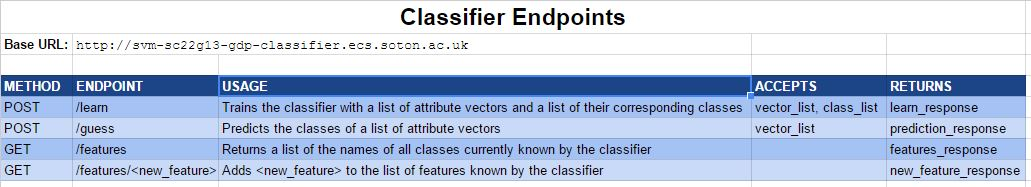
\includegraphics[width=\textwidth]{figs/4/classifier_endpoints}
    \caption{ Endpoint Reference Contract extract for the Classifier}
    \label{fig:classifier_endpoints}
\end{figure}